\hypertarget{patStats_8c}{
\section{pat\-Stats.c File Reference}
\label{patStats_8c}\index{patStats.c@{patStats.c}}
}
{\tt \#include $<$math.h$>$}\par
{\tt \#include \char`\"{}pat\-Stats.h\char`\"{}}\par


Include dependency graph for pat\-Stats.c:\begin{figure}[H]
\begin{center}
\leavevmode
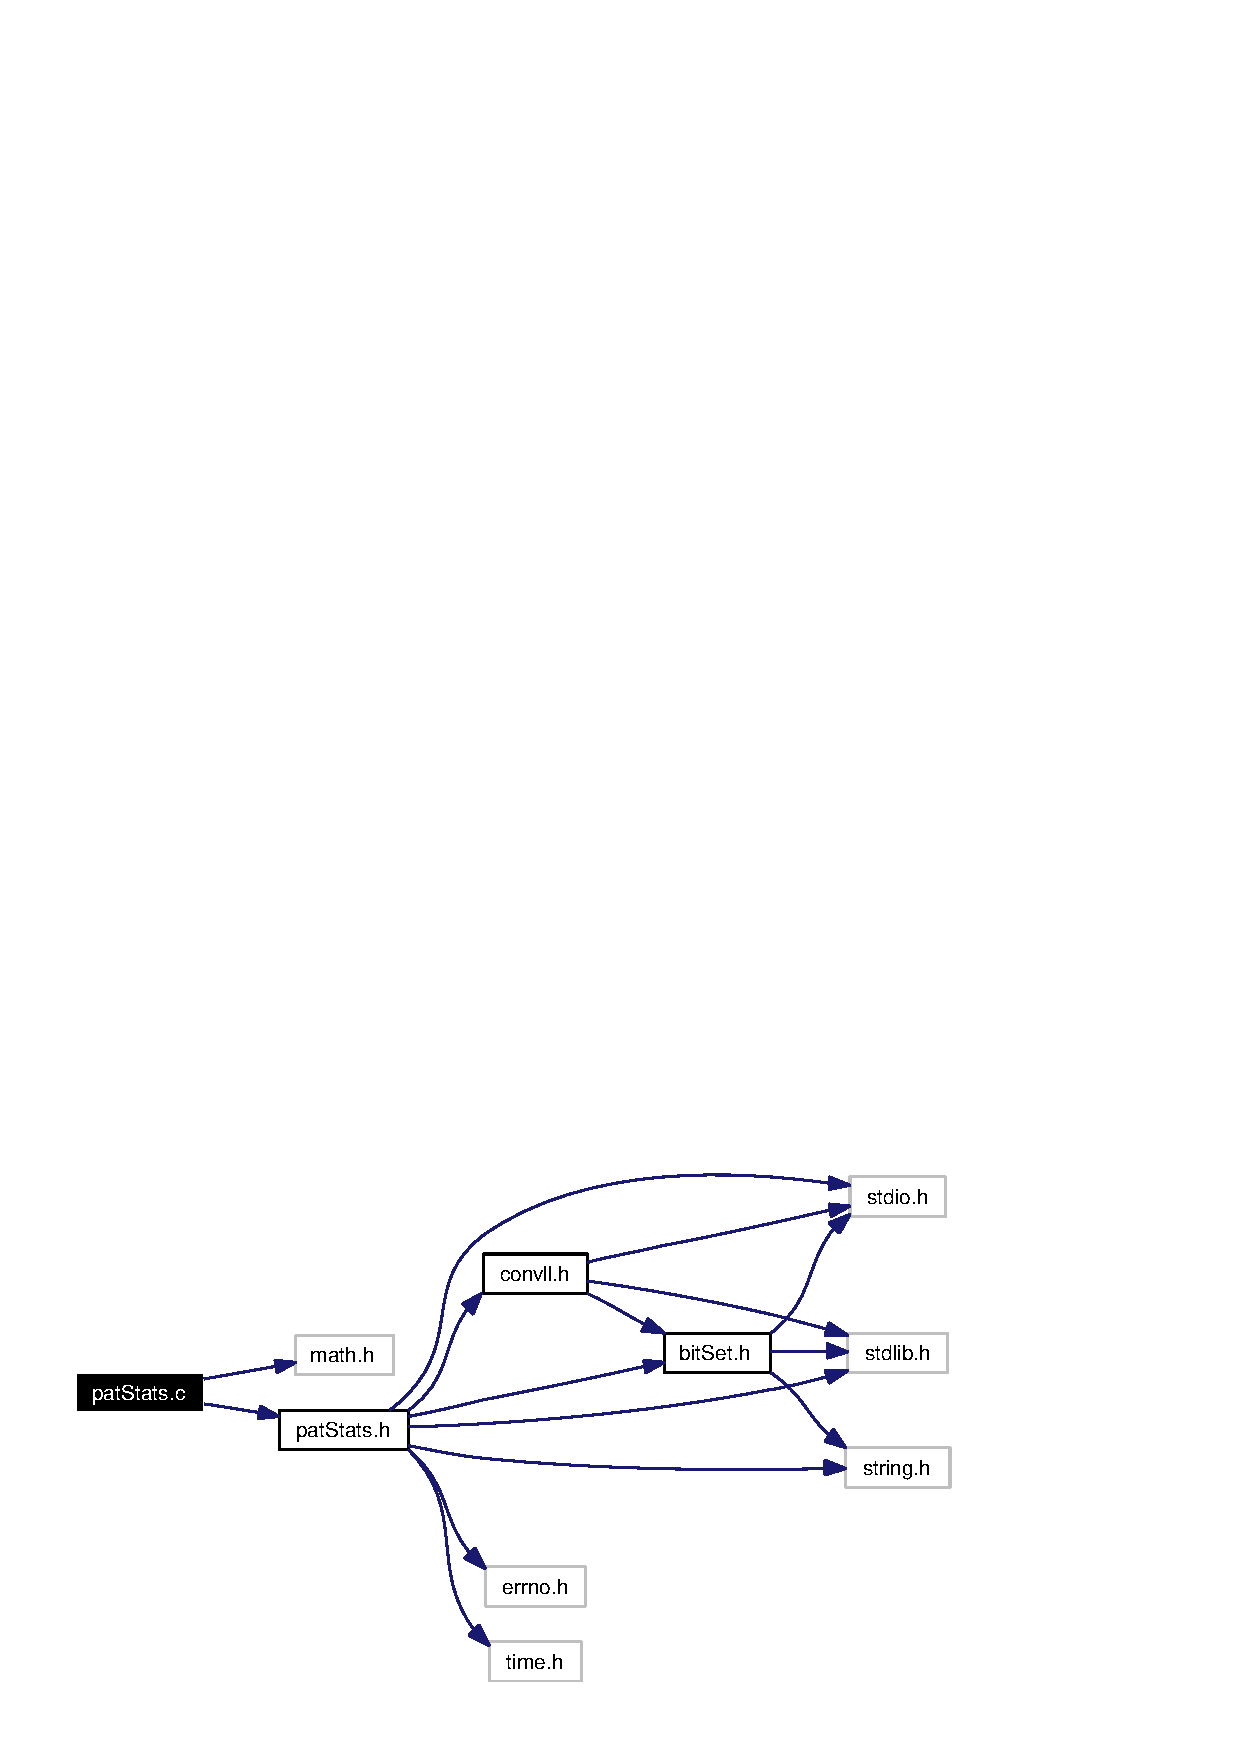
\includegraphics[width=228pt]{patStats_8c__incl}
\end{center}
\end{figure}
\subsection*{Functions}
\begin{CompactItemize}
\item 
int \hyperlink{patStats_8c_a0}{get\-Largest\-Support} (\hyperlink{structcnode}{cll\_\-t} $\ast$cliqs)
\item 
int \hyperlink{patStats_8c_a1}{get\-Largest\-Length} (\hyperlink{structcnode}{cll\_\-t} $\ast$cliqs)
\item 
int \hyperlink{patStats_8c_a2}{measure\-Diagonal} (const \hyperlink{structbitGraph__t}{bit\-Graph\_\-t} $\ast$bg, const int i, const int j)
\item 
unsigned int $\ast$$\ast$ \hyperlink{patStats_8c_a3}{increase\-Mem} (unsigned int $\ast$$\ast$d, int dim\-To\-Change, int curr\-Support, int curr\-Length, int new\-Val)
\item 
unsigned int $\ast$$\ast$ \hyperlink{patStats_8c_a4}{old\-Get\-Stat\-Mat} (\hyperlink{structbitGraph__t}{bit\-Graph\_\-t} $\ast$bg, int support, int length, int $\ast$support\-Dim, int $\ast$length\-Dim, int num\-Blanks)
\item 
unsigned int $\ast$$\ast$ \hyperlink{patStats_8c_a5}{get\-Stat\-Mat} (\hyperlink{structbitGraph__t}{bit\-Graph\_\-t} $\ast$bg, int support, int length, int $\ast$support\-Dim, int $\ast$length\-Dim, int num\-Blanks, int s, FILE $\ast$OUTPUT\_\-FILE)
\item 
int \hyperlink{patStats_8c_a6}{cum\-DMatrix} (unsigned int $\ast$$\ast$d, \hyperlink{structcnode}{cll\_\-t} $\ast$cliqs, int curr\-Support, int curr\-Length, int bg\-Size, int num\-Seqs)
\item 
double \hyperlink{patStats_8c_a7}{calc\-Stat\-Cliq} (unsigned int $\ast$$\ast$d, \hyperlink{structcnode}{cll\_\-t} $\ast$cliq, int num\-Windows)
\item 
int \hyperlink{patStats_8c_a8}{calc\-Stat\-All\-Cliqs} (unsigned int $\ast$$\ast$d, \hyperlink{structcnode}{cll\_\-t} $\ast$all\-Cliqs, int num\-Windows)
\item 
int \hyperlink{patStats_8c_a9}{free\-D} (unsigned int $\ast$$\ast$d, int support\-Dim)
\item 
int \hyperlink{patStats_8c_a10}{stat\-Compare} (const \hyperlink{structcnode}{cll\_\-t} $\ast$$\ast$first, const \hyperlink{structcnode}{cll\_\-t} $\ast$$\ast$second)
\item 
\hyperlink{structcnode}{cll\_\-t} $\ast$ \hyperlink{patStats_8c_a11}{sort\-By\-Stats} (\hyperlink{structcnode}{cll\_\-t} $\ast$all\-Cliqs)
\end{CompactItemize}


\subsection*{Detailed Description}
This file defines functions that are used to compute the statistical significance of motifs for both the sequence based and real value based implementations of Gemoda. The basic approach we take, is to calculate the probability of establishing a single cluster, and to multiply this probability by the probability that the cluster can be extended an arbitrary number of locations. Essentially, this is the probability of getting and elementary motif during the clustering phase and having that motif convolved multiple times during the convolution phase.

Definition in file \hyperlink{patStats_8c-source}{pat\-Stats.c}.

\subsection*{Function Documentation}
\hypertarget{patStats_8c_a8}{
\index{patStats.c@{pat\-Stats.c}!calcStatAllCliqs@{calcStatAllCliqs}}
\index{calcStatAllCliqs@{calcStatAllCliqs}!patStats.c@{pat\-Stats.c}}
\subsubsection[calcStatAllCliqs]{\setlength{\rightskip}{0pt plus 5cm}int calc\-Stat\-All\-Cliqs (unsigned int $\ast$$\ast$ {\em d}, \hyperlink{structcnode}{cll\_\-t} $\ast$ {\em all\-Cliqs}, int {\em num\-Windows})}}
\label{patStats_8c_a8}




Definition at line 676 of file pat\-Stats.c.

References calc\-Stat\-Cliq(), cnode::next, and cnode::stat.

Referenced by main().

\scriptsize\begin{verbatim}677 {
678   cll_t * curr = NULL;
679   curr = allCliqs;
680   while (curr != NULL)
681     {
682       curr->stat = calcStatCliq (d, curr, numWindows);
683       curr = curr->next;
684     }
685   return (0);
686 }
\end{verbatim}
\normalsize 


\hypertarget{patStats_8c_a7}{
\index{patStats.c@{pat\-Stats.c}!calcStatCliq@{calcStatCliq}}
\index{calcStatCliq@{calcStatCliq}!patStats.c@{pat\-Stats.c}}
\subsubsection[calcStatCliq]{\setlength{\rightskip}{0pt plus 5cm}double calc\-Stat\-Cliq (unsigned int $\ast$$\ast$ {\em d}, \hyperlink{structcnode}{cll\_\-t} $\ast$ {\em cliq}, int {\em num\-Windows})}}
\label{patStats_8c_a7}




Definition at line 623 of file pat\-Stats.c.

References cnode::length, cnode::set, and c\-Set\_\-t::size.

Referenced by calc\-Stat\-All\-Cliqs().

\scriptsize\begin{verbatim}624 {
625   double stat = 0;
626   int i = 0;
627   int supChooseTwo = 0;
628   double interimP = 0;
629   int support = cliq->set->size;
630   int length = cliq->length;
631   double numTrials = 0;
632   if (support < 2)
633     {
634       fprintf (stderr, "Support for cluster less than 2... exiting.\n");
635       fflush (stderr);
636       exit (0);
637     }
638   
639     // OK, so support is at least two.  So we make the connections all
640     // on the first level, knowing that each node being connected has
641     // at least zero in common.  There are [(size of cluster) - 1] of
642     // these connections to be made.
643     // And we know we can call for d[0][1] because if the second index
644     // were out of bounds, then there would be no similarities, and
645     // there would be no reason to call this function.
646     interimP = ((double) d[0][1]) / ((double) d[0][0]);
647   stat = pow (interimP, support - 1);
648   stat *= ((double) numWindows * (numWindows - 1)) / ((double) 2);
649   
650     // Now we actually calculate the probability... the first connection
651     // has to be made no matter what, and after that we multiply for 
652     // every connection after the first one.  So we descend iteratively
653     // until we have made all connections, terminating after we've made
654     // the single i = (n - 2) connection.  There is no i = (n - 1) 
655     // connection.
656     for (i = 1; i < support - 1; i++)
657     {
658       interimP = ((double) d[i][1]) / ((double) d[i][0]);
659       stat *= pow (interimP, support - i - 1);
660       stat *= ((double) (numWindows - (i + 1))) / ((double) (i + 2));
661     } supChooseTwo = (support * (support - 1)) / 2;
662   
663     // Remember that length = (numwindows - 1), or alternatively,
664     // the number of extensions... normally we'd want to have the last
665     // p be p[support][numwindows - 1], which corresponds to 
666     // alteredD[support][numwindows]/alteredD[support][numwindows-1],
667     // so that means we want our last d to be d[support][numwindows].
668     // Here, we note that the calculation of p's would be continuously
669     // re-normalizing, so multiplying all p's is the same as dividing
670     // the last d by the initial d.
671     interimP = ((double) d[support][length + 1]) / ((double) d[support][1]);
672   stat *= pow (interimP, supChooseTwo);
673   return stat;
674 }
\end{verbatim}
\normalsize 


\hypertarget{patStats_8c_a6}{
\index{patStats.c@{pat\-Stats.c}!cumDMatrix@{cumDMatrix}}
\index{cumDMatrix@{cumDMatrix}!patStats.c@{pat\-Stats.c}}
\subsubsection[cumDMatrix]{\setlength{\rightskip}{0pt plus 5cm}int cum\-DMatrix (unsigned int $\ast$$\ast$ {\em d}, \hyperlink{structcnode}{cll\_\-t} $\ast$ {\em cliqs}, int {\em curr\-Support}, int {\em curr\-Length}, int {\em bg\-Size}, int {\em num\-Seqs})}}
\label{patStats_8c_a6}




Definition at line 522 of file pat\-Stats.c.

References get\-Largest\-Length(), and get\-Largest\-Support().

Referenced by main().

\scriptsize\begin{verbatim}524 {
525   int maxSup = 0;
526   int maxLen = 0;
527   int i, j;
528   int numWins = 0;
529   
530     maxSup = getLargestSupport (cliqs);
531   maxLen = getLargestLength (cliqs);
532   
533 /********* COMMENTED OUT
534     // First we note that the number of unique streaks of a given
535     //  support is defined by d[support][1], where as 1 increases,
536     //  the value of d decreases because only unique streaks are
537     //  counted.
538     // We also note that the number of disjoint node-pairs with a given
539     //  number of other nodes in common is defined by d[support][0].
540     // So, in order to properly account for all "unique" comparisons 
541     //  (which is equal to (# streaks + # disjoint node-pairs), we must
542     //  add d[support][1] to d[support][0].
543     
544     for (i = 0; i < currSupport + 1; i++) {
545         d[i][0] += d[i][1];
546     }
547     ********************/ 
548     
549     // We no longer need to do that, since now we sum across both
550     // the support and the length dimensions.  Now, d[support][0] will
551     // necessarily include d[support][1] being added to it.  We don't 
552     // want to add this anymore, otherwise we would be underestimating
553     // the probability of making that first connection.  For instance,
554     // if there were no nodes with 20 in common that weren't also 
555     // connected, and no nodes whatsoever with more than 20 in common,
556     // we'd want the p[20][0] to be 1, which would be 
557     // d[20][1]/d[20][0].  When summing across length directions,
558     // this happens naturally, whereas before we needed to do it 
559     // artificially as per above.  If we did above, we'd have the
560     // probability of each node being 1/2 instead of 1.
561     
562     // Rather than storing doubles and doing lots of multiplications,
563     // we're going to limit the number of operations done in the actual
564     // probability calculation by only storing cumulative sums in d.
565     // Now remember, what we're storing at each location is the 
566     // number of nodes with [i] or more nodes in common (including
567     // each other and selves) that can be extended [j] times (with
568     // their initial similarity counting as 1).
569     // 
570     // We go up to the last possible index in the length direction, which
571     // means going up to [maxLen].  We know that this is legitimate
572     // because maxLen is less than or equal to the longest possible 
573     // diagonal, and the longest possible diagonal will be less
574     // than or equal to currLength.  Since we have allotted 
575     // (currLength + 1) integers, we know we're OK to access [currLength].
576     for (j = 0; j < currLength + 1; j++)
577     {
578       
579     // We start at currSupport - 1, because currSupport will
580     // clearly not be changed, and this makes it a much easier
581     // loop to read.
582     for (i = currSupport - 1; i >= 0; i--)
583     {
584       d[i][j] += d[i + 1][j];
585     }
586     }
587   for (i = 0; i < currSupport + 1; i++)
588     {
589       for (j = currLength - 1; j >= 0; j--)
590     {
591       d[i][j] += d[i][j + 1];
592     }
593     }
594   
595     // Now we need to forcibly set d[0][0] to its correct value... it's 
596     // just the total number of comparisons, not including comparisons
597     // to delimiter 0's meant to separate sequences.  The number of 
598     // windows is equal to the number of offsets minus the number
599     // of sequences (assuming one delimiter per sequence).  We don't count
600     // the main diagonal, so the first row has one less, and we want to
601     // sum over all the subsequent rows in the upper half of the matrix.
602     // So it's (numWins - 1)*(numWins - 1 + 1)/2 to sum that up.
603     numWins = bgSize - numSeqs;
604   d[0][0] = numWins * (numWins - 1) / 2;
605   
606     /*
607         for (i = 0; i <= maxSup; i++) { printf("support = %d:\t",i); for (j = 0; j <=
608        maxLen; j++) { printf("%d\t",d[i][j]); } printf("\n"); } 
609      */ 
610     return 1;
611 }
\end{verbatim}
\normalsize 


\hypertarget{patStats_8c_a9}{
\index{patStats.c@{pat\-Stats.c}!freeD@{freeD}}
\index{freeD@{freeD}!patStats.c@{pat\-Stats.c}}
\subsubsection[freeD]{\setlength{\rightskip}{0pt plus 5cm}int free\-D (unsigned int $\ast$$\ast$ {\em d}, int {\em support\-Dim})}}
\label{patStats_8c_a9}




Definition at line 688 of file pat\-Stats.c.

Referenced by main().

\scriptsize\begin{verbatim}689 {
690   int i = 0;
691   if (d == 0)
692     {
693       return 0;
694     }
695   else
696     {
697       
698     // Still, it's supportDim + 1, because we have an extra
699     // one for the "0" support.
700     for (i = 0; i < supportDim + 1; i++)
701     {
702       free (d[i]);
703     }
704       free (d);
705       return 0;
706     }
707 }
\end{verbatim}
\normalsize 


\hypertarget{patStats_8c_a1}{
\index{patStats.c@{pat\-Stats.c}!getLargestLength@{getLargestLength}}
\index{getLargestLength@{getLargestLength}!patStats.c@{pat\-Stats.c}}
\subsubsection[getLargestLength]{\setlength{\rightskip}{0pt plus 5cm}int get\-Largest\-Length (\hyperlink{structcnode}{cll\_\-t} $\ast$ {\em cliqs})}}
\label{patStats_8c_a1}


Given a clique linked list, this function will return an integer which is equal to the length of the member of the linked list with the largest length.

Definition at line 44 of file pat\-Stats.c.

References cnode::length, and cnode::next.

Referenced by cum\-DMatrix().

\scriptsize\begin{verbatim}45 {
46   int len = 0;
47   cll_t * curCliq = NULL;
48   curCliq = cliqs;
49   while (curCliq != NULL)
50     {
51       if (curCliq->length > len)
52     {
53       len = curCliq->length;
54     }
55       curCliq = curCliq->next;
56     }
57   
58     // We return (len + 1) because the length of the shortest streak
59     // is one, but is stored in the cluster data structure as being
60     // zero (number of extensions that have been made).
61     return (len + 1);
62 }
\end{verbatim}
\normalsize 


\hypertarget{patStats_8c_a0}{
\index{patStats.c@{pat\-Stats.c}!getLargestSupport@{getLargestSupport}}
\index{getLargestSupport@{getLargestSupport}!patStats.c@{pat\-Stats.c}}
\subsubsection[getLargestSupport]{\setlength{\rightskip}{0pt plus 5cm}int get\-Largest\-Support (\hyperlink{structcnode}{cll\_\-t} $\ast$ {\em cliqs})}}
\label{patStats_8c_a0}


Given a clique linked list, this function will return an integer which is equal to the support of the member of the linked list with the largest support.

Definition at line 22 of file pat\-Stats.c.

References cnode::next, cnode::set, and c\-Set\_\-t::size.

Referenced by cum\-DMatrix().

\scriptsize\begin{verbatim}23 {
24   int size = 0;
25   cll_t * curCliq = NULL;
26   curCliq = cliqs;
27   while (curCliq != NULL)
28     {
29       if (curCliq->set->size > size)
30     {
31       size = curCliq->set->size;
32     }
33       curCliq = curCliq->next;
34     }
35   return size;
36 }
\end{verbatim}
\normalsize 


\hypertarget{patStats_8c_a5}{
\index{patStats.c@{pat\-Stats.c}!getStatMat@{getStatMat}}
\index{getStatMat@{getStatMat}!patStats.c@{pat\-Stats.c}}
\subsubsection[getStatMat]{\setlength{\rightskip}{0pt plus 5cm}unsigned int$\ast$$\ast$ get\-Stat\-Mat (\hyperlink{structbitGraph__t}{bit\-Graph\_\-t} $\ast$ {\em bg}, int {\em support}, int {\em length}, int $\ast$ {\em support\-Dim}, int $\ast$ {\em length\-Dim}, int {\em num\-Blanks}, int {\em s}, FILE $\ast$ {\em OUTPUT\_\-FILE})}}
\label{patStats_8c_a5}




Definition at line 329 of file pat\-Stats.c.

References bit\-Graph\-Row\-Intersection(), check\-Bit(), count\-Set(), delete\-Bit\-Set(), bit\-Graph\_\-t::graph, increase\-Mem(), measure\-Diagonal(), new\-Bit\-Set(), next\-Bit\-Bit\-Set(), and bit\-Graph\_\-t::size.

Referenced by main().

\scriptsize\begin{verbatim}331 {
332   int *Q = NULL;
333   unsigned int **d = NULL;
334   int i, j, k;
335   int x, y;
336   bitSet_t * X = NULL;
337   int currSupport;
338   int currLength;
339   int multiplier = 50;
340   int diagonal = 0;
341   time_t probStart, probEnd;
342   int timeNeeded = 0;
343   int sampleCounter = 1;
344   
345     // int visitCounter = 0, uniqCounter = 0;
346     currSupport = support * multiplier;
347   currLength = length * multiplier;
348   X = newBitSet (bg->size);
349   
350     // printf("Made bitSet of size %d\n", bg->size);
351     Q = (int *) malloc (bg->size * sizeof (int));
352   if (Q == NULL)
353     {
354       fprintf (stderr,
355         "\nMemory error --- couldn't allocate array!"  "\n%s\n",
356         strerror (errno));
357       fflush (stderr);
358       exit (0);
359     }
360   for (i = 0; i < bg->size; i++)
361     {
362       Q[i] = 0;
363     }
364   d =
365     (unsigned int **) malloc ((currSupport + 1) * sizeof (unsigned int *));
366   if (d == NULL)
367     {
368       fprintf (stderr,
369         "\nMemory error --- couldn't allocate array!"  "\n%s\n",
370         strerror (errno));
371       fflush (stderr);
372       exit (0);
373     }
374   for (i = 0; i < currSupport + 1; i++)
375     {
376       d[i] =
377     (unsigned int *) malloc ((currLength + 1) * sizeof (unsigned int));
378       if (d[i] == NULL)
379     {
380       fprintf (stderr, "\nMemory error --- couldn't allocate array!" 
381             "\n%s\n", strerror (errno));
382       fflush (stderr);
383       exit (0);
384     }
385       for (j = 0; j < currLength + 1; j++)
386     {
387       d[i][j] = 0;
388     }
389     }
390   
391     // printf("size=%d\n",bg->size);
392     time (&probStart);
393   for (i = 0; i < bg->size; i++)
394     {
395       if (i == 200)
396     {
397       time (&probEnd);
398       timeNeeded = ((double) (probEnd - probStart)) / 
399         ((double) 60) * ((double) bg->size) / ((double) 200);
400       if (timeNeeded > 2)
401         {
402           fprintf (OUTPUT_FILE,
403             "Max total time to calculate probability:\n");
404           fprintf (OUTPUT_FILE, "\t%d minutes\n", timeNeeded);
405           fprintf (OUTPUT_FILE, "Actual time will be less than this, " 
406             "but at least half of it.\n");
407           fprintf (OUTPUT_FILE,
408             "To bypass excessive probability calculations," 
409             " cancel and use a different value\n" 
410             " for the '-s' flag (samples every " 
411             "'s' points).\n");
412           fflush (NULL);
413         }
414     }
415       j = nextBitBitSet (bg->graph[i], 0);
416       while (j >= 0)
417     {
418       k = nextBitBitSet (bg->graph[i], j + 1);
419       while (k >= 0)
420         {
421           if (checkBit (bg->graph[j], k) == 0)
422         {
423           if (sampleCounter == s)
424             {
425               bitGraphRowIntersection (bg, j, k, X);
426               
427             // visitCounter++;
428             if (nextBitBitSet (X, 0) >= i)
429             {
430               
431                 // uniqCounter++;
432                 x = countSet (X);
433               while (x > currSupport)
434                 {
435                   d =
436                 increaseMem (d, 1, currSupport, currLength,
437                          currSupport +
438                          support * multiplier);
439                   currSupport += support * multiplier;
440                 }
441               d[x][0] += 1;
442             }
443               sampleCounter = 0;
444             }
445           sampleCounter++;
446         }
447           k = nextBitBitSet (bg->graph[i], k + 1);
448         }
449       if (j <= i)
450         {
451           j = nextBitBitSet (bg->graph[i], j + 1);
452           continue;
453         }
454       bitGraphRowIntersection (bg, i, j, X);
455       x = countSet (X);
456       
457         // Note, now we're using "diagonals" rather than
458         // location in a horizontal array.  So you always
459         // start from the main diagonal at 0 and move out.
460         diagonal = j - i;
461       
462         // We change this to greater-than-one because
463         // after Q[diagonal] is reduced to one, it isn't 
464         // visited again until we reach a new streak, (because
465         // the next bit in the diagonal is a zero), and at
466         // that point we want to start with a new diagonal
467         // measure.
468         if (Q[diagonal] > 1)
469         {
470           y = Q[diagonal] - 1;
471           Q[diagonal]--;
472         }
473       else
474         {
475           y = measureDiagonal (bg, i, j);
476           Q[diagonal] = y;
477         }
478       while (x > currSupport)
479         {
480           d = increaseMem (d, 1, currSupport, currLength,
481                 currSupport + support * multiplier);
482           currSupport += support * multiplier;
483         }
484       while (y > currLength)
485         {
486           d =
487         increaseMem (d, 2, currSupport, currLength,
488                  currLength + length * multiplier);
489           currLength += length * multiplier;
490         }
491       d[x][y]++;
492       j = nextBitBitSet (bg->graph[i], j + 1);
493       
494         /*
495             if(x != 0){ printf("%d:\t%d %d\n", j, x, y); fflush(stdout); } 
496          */ 
497     }
498       
499     /*
500         printf("done\n"); fflush(stdout); 
501      */ 
502     }
503   
504     // We need to rescale by the sampling factor for all i>0 in d[i][0].
505     // 
506     for (i = 1; i < currSupport; i++)
507     {
508       d[i][0] *= s;
509     }
510   
511     // Now we only need to assign the correct value for d[0][0]...
512     // but rather than figuring that out, we will just assign it in the
513     // cumulative function, since there it is merely the number of unique
514     // non-self comparisons and is easy to calculate.
515     deleteBitSet (X);
516   free (Q);
517   *supportDim = currSupport;
518   *lengthDim = currLength;
519   return (d);
520 }
\end{verbatim}
\normalsize 


\hypertarget{patStats_8c_a3}{
\index{patStats.c@{pat\-Stats.c}!increaseMem@{increaseMem}}
\index{increaseMem@{increaseMem}!patStats.c@{pat\-Stats.c}}
\subsubsection[increaseMem]{\setlength{\rightskip}{0pt plus 5cm}unsigned int$\ast$$\ast$ increase\-Mem (unsigned int $\ast$$\ast$ {\em d}, int {\em dim\-To\-Change}, int {\em curr\-Support}, int {\em curr\-Length}, int {\em new\-Val})}}
\label{patStats_8c_a3}


This function is used to increase the size of an array of pointers to pointers to integers. dim\-To\-Change is 1 for the first dimension (support), 2 for the second dimension (length). new\-Val is the new value for the dimension to be changed, not including the \char`\"{}1\char`\"{} that should be added... so it should just be some integer times the initial support.

Definition at line 91 of file pat\-Stats.c.

Referenced by get\-Stat\-Mat(), and old\-Get\-Stat\-Mat().

\scriptsize\begin{verbatim}93 {
94   int i = 0, j = 0;
95   if (dimToChange == 1)
96     {
97       d =
98     (unsigned int **) realloc (d, (newVal + 1) * sizeof (unsigned int *));
99       if (d == NULL)
100     {
101       fprintf (stderr, "\nMemory error --- couldn't allocate array!" 
102             "\n%s\n", strerror (errno));
103       fflush (stderr);
104       exit (0);
105     }
106       for (i = currSupport + 1; i < newVal + 1; i++)
107     {
108       d[i] =
109         (unsigned int *) malloc ((currLength + 1) *
110                      sizeof (unsigned int));
111       if (d[i] == NULL)
112         {
113           fprintf (stderr,
114             "\nMemory error --- couldn't allocate array!" 
115             "\n%s\n", strerror (errno));
116           fflush (stderr);
117           exit (0);
118         }
119       for (j = 0; j < currLength + 1; j++)
120         {
121           d[i][j] = 0;
122         }
123     }
124       return d;
125     }
126   else if (dimToChange == 2)
127     {
128       for (i = 0; i < currSupport + 1; i++)
129     {
130       d[i] =
131         (unsigned int *) realloc (d[i],
132                       (newVal + 1) * sizeof (unsigned int));
133       if (d[i] == NULL)
134         {
135           fprintf (stderr,
136             "\nMemory error --- couldn't allocate array!" 
137             "\n%s\n", strerror (errno));
138           fflush (stderr);
139           exit (0);
140         }
141       for (j = currLength + 1; j < newVal + 1; j++)
142         {
143           d[i][j] = 0;
144         }
145     }
146       return d;
147     }
148   else
149     {
150       fprintf (stderr, "Invalid arguments to increaseMem!\n\n");
151       fflush (stderr);
152       exit (0);
153     }
154 }
\end{verbatim}
\normalsize 


\hypertarget{patStats_8c_a2}{
\index{patStats.c@{pat\-Stats.c}!measureDiagonal@{measureDiagonal}}
\index{measureDiagonal@{measureDiagonal}!patStats.c@{pat\-Stats.c}}
\subsubsection[measureDiagonal]{\setlength{\rightskip}{0pt plus 5cm}int measure\-Diagonal (const \hyperlink{structbitGraph__t}{bit\-Graph\_\-t} $\ast$ {\em bg}, const int {\em i}, const int {\em j})}}
\label{patStats_8c_a2}


Given a bit graph, and two indices within that bit graph, this will return an integer which is equal to the number of values in the bit graph that are true along a diagonal that begins at the two indices. This routine is used to check for streaks in an adjacency matrix and is used during the convolution.

Definition at line 72 of file pat\-Stats.c.

References bit\-Graph\-Check\-Bit().

Referenced by get\-Stat\-Mat(), and old\-Get\-Stat\-Mat().

\scriptsize\begin{verbatim}73 {
74   int len = 0;
75   while (bitGraphCheckBit (bg, i + len, j + len) != 0)
76     {
77       len++;
78     }
79   return len;
80 }
\end{verbatim}
\normalsize 


\hypertarget{patStats_8c_a4}{
\index{patStats.c@{pat\-Stats.c}!oldGetStatMat@{oldGetStatMat}}
\index{oldGetStatMat@{oldGetStatMat}!patStats.c@{pat\-Stats.c}}
\subsubsection[oldGetStatMat]{\setlength{\rightskip}{0pt plus 5cm}unsigned int$\ast$$\ast$ old\-Get\-Stat\-Mat (\hyperlink{structbitGraph__t}{bit\-Graph\_\-t} $\ast$ {\em bg}, int {\em support}, int {\em length}, int $\ast$ {\em support\-Dim}, int $\ast$ {\em length\-Dim}, int {\em num\-Blanks})}}
\label{patStats_8c_a4}


OK, here is something that is a little bit \char`\"{}hackish\char`\"{} but that we have to do. Since our initial matrix is being pruned and filtered before being clustered, but we need to calculate stats based on the original matrix, we need to get information from the matrix before pruning, so we're using this function. We could just make a copy of that matrix, but it's far too big, and that would cause an unneccessary constraint on memory, limiting the size of problems we can address. But we need to define just how big our d matrix is before we can use it. We could go through and compute the longest streak beforehand, and then redo everything, but we've already found the first step of finding all of the streaks to be fairly expensive (KLJ). So instead what we'll do is use the user's parameters as a benchmark and expand from there. We'll assume that most of the time, the biggest streak (number of extensions) will be less than 50 times the length given as input by the user, and the biggest support will be less than 50 times the minimum number of support given by the user. This seems perhaps overly conservative, but otherwise is reasonable. We then realize that even on a 64-bit computer, if the user gives L=50 and K=50, we'll still use less than 48 MB of memory... and if L=50 and K=50, it is extremely likely that doubling the adjacency matrix would have been a much worse option. Scaling back to more common values of L$\sim$20 and K$\sim$20, the memory used shoots down to $\sim$9MB, which is definitely acceptable. Now, if for some reason our initial allocation wasn't enough, then we'll have to go through and realloc all of our memory again. Somewhat time-consuming, but hopefully not done too often. Each time we find we try to put something in an index that doesn't exist, we'll reallocate our memory, adding twice as much in the dimension that was violated. It is important to us that we get back the final dimensions of this matrix, since in the support dimension we'll have to sum across all values, and in the length dimension we'll have to be sure we're not at the edge of a matrix during our d manipulations later on.

Definition at line 196 of file pat\-Stats.c.

References bit\-Graph\-Row\-Intersection(), count\-Set(), delete\-Bit\-Set(), increase\-Mem(), measure\-Diagonal(), new\-Bit\-Set(), and bit\-Graph\_\-t::size.

\scriptsize\begin{verbatim}198 {
199   int *Q = NULL;
200   unsigned int **d = NULL;
201   int i, j;
202   int x, y;
203   bitSet_t * X = NULL;
204   int currSupport;
205   int currLength;
206   int multiplier = 50;
207   time_t probStart, probEnd;
208   int timeNeeded = 0;
209   currSupport = support * multiplier;
210   currLength = length * multiplier;
211   X = newBitSet (bg->size);
212   
213     // printf("Made bitSet of size %d\n", bg->size);
214     Q = (int *) malloc (bg->size * sizeof (int));
215   if (Q == NULL)
216     {
217       fprintf (stderr,
218         "\nMemory error --- couldn't allocate array!"  "\n%s\n",
219         strerror (errno));
220       fflush (stderr);
221       exit (0);
222     }
223   for (i = 0; i < bg->size; i++)
224     {
225       Q[i] = 0;
226     }
227   d =
228     (unsigned int **) malloc ((currSupport + 1) * sizeof (unsigned int *));
229   if (d == NULL)
230     {
231       fprintf (stderr,
232         "\nMemory error --- couldn't allocate array!"  "\n%s\n",
233         strerror (errno));
234       fflush (stderr);
235       exit (0);
236     }
237   for (i = 0; i < currSupport + 1; i++)
238     {
239       d[i] =
240     (unsigned int *) malloc ((currLength + 1) * sizeof (unsigned int));
241       if (d[i] == NULL)
242     {
243       fprintf (stderr, "\nMemory error --- couldn't allocate array!" 
244             "\n%s\n", strerror (errno));
245       fflush (stderr);
246       exit (0);
247     }
248       for (j = 0; j < currLength + 1; j++)
249     {
250       d[i][j] = 0;
251     }
252     }
253   time (&probStart);
254   for (i = 0; i < bg->size; i++)
255     {
256       if (i == 200)
257     {
258       time (&probEnd);
259       timeNeeded = ((double) (probEnd - probStart)) / 
260         ((double) 60) * ((double) bg->size) / ((double) 200);
261       if (timeNeeded > 2)
262         {
263           printf ("Max total time to calculate probability:\n");
264           printf ("\t%d minutes\n", timeNeeded);
265           printf ("Actual time will be less than this, but at",
266                "least half of it.\n");
267           printf ("To bypass excessive probability calculations,",
268                "cancel and use the '-d' flag.\n");
269           fflush (NULL);
270         }
271     }
272       for (j = bg->size - 1; j > i; j--)
273     {
274       bitGraphRowIntersection (bg, i, j, X);
275       x = countSet (X);
276       if (Q[j - 1] != 0)
277         {
278           y = Q[j - 1] - 1;
279           Q[j] = Q[j - 1] - 1;
280         }
281       else
282         {
283           y = measureDiagonal (bg, i, j);
284           Q[j] = y;
285         }
286       while (x > currSupport)
287         {
288           d = increaseMem (d, 1, currSupport, currLength,
289                 currSupport + support * multiplier);
290           currSupport += support * multiplier;
291         }
292       while (y > currLength)
293         {
294           d =
295         increaseMem (d, 2, currSupport, currLength,
296                  currLength + length * multiplier);
297           currLength += length * multiplier;
298         }
299       d[x][y]++;
300       
301         /*
302             if(x != 0){ printf("%d:\t%d %d\n", j, x, y); fflush(stdout); } 
303          */ 
304     }
305       
306     /*
307         printf("done\n"); fflush(stdout); 
308      */ 
309     }
310   
311     // We know that the "blanks", inserted to delimit unique sequences
312     // and prevent convolution through them, will skew our statistics,
313     // so we subtract them.  We know that they will never be similar to
314     // any others, so will only add to the d[0][0] number.  Furthermore,
315     // we know how many they add.  Since d never hits the main diagonal
316     // and only does the upper half of the matrix, the first one 
317     // contributes bgsize - 1 to d[0][0], the next bgsize - 2, etc.
318     for (i = 0; i < numBlanks; i++)
319     {
320       d[0][0] -= bg->size - 1 - i;
321     }
322   deleteBitSet (X);
323   free (Q);
324   *supportDim = currSupport;
325   *lengthDim = currLength;
326   return (d);
327 }
\end{verbatim}
\normalsize 


\hypertarget{patStats_8c_a11}{
\index{patStats.c@{pat\-Stats.c}!sortByStats@{sortByStats}}
\index{sortByStats@{sortByStats}!patStats.c@{pat\-Stats.c}}
\subsubsection[sortByStats]{\setlength{\rightskip}{0pt plus 5cm}\hyperlink{structcnode}{cll\_\-t}$\ast$ sort\-By\-Stats (\hyperlink{structcnode}{cll\_\-t} $\ast$ {\em all\-Cliqs})}}
\label{patStats_8c_a11}


This function is used to sort a link to list of cliques by the statistical significance of the motifs found in that linked list.

Definition at line 732 of file pat\-Stats.c.

References cnode::id, cnode::next, and stat\-Compare().

Referenced by main().

\scriptsize\begin{verbatim}733 {
734   cll_t * curCliq = NULL;
735   cll_t ** arrayOfCliqs = NULL;
736   int numOfCliqs = 0;
737   int i = 0;
738   curCliq = allCliqs;
739   if (curCliq != NULL)
740     {
741       numOfCliqs = curCliq->id + 1;
742     }
743   else
744     {
745       return (NULL);
746     }
747   arrayOfCliqs = (cll_t **) malloc (numOfCliqs * sizeof (cll_t *));
748   for (i = 0; i < numOfCliqs; i++)
749     {
750       arrayOfCliqs[i] = curCliq;
751       curCliq = curCliq->next;
752     }
753   qsort (arrayOfCliqs, numOfCliqs, sizeof (cll_t *), statCompare);
754   for (i = 0; i < numOfCliqs - 1; i++)
755     {
756       arrayOfCliqs[i]->next = arrayOfCliqs[i + 1];
757     }
758   arrayOfCliqs[numOfCliqs - 1]->next = NULL;
759   return (arrayOfCliqs[0]);
760 }
\end{verbatim}
\normalsize 


\hypertarget{patStats_8c_a10}{
\index{patStats.c@{pat\-Stats.c}!statCompare@{statCompare}}
\index{statCompare@{statCompare}!patStats.c@{pat\-Stats.c}}
\subsubsection[statCompare]{\setlength{\rightskip}{0pt plus 5cm}int stat\-Compare (const \hyperlink{structcnode}{cll\_\-t} $\ast$$\ast$ {\em first}, const \hyperlink{structcnode}{cll\_\-t} $\ast$$\ast$ {\em second})}}
\label{patStats_8c_a10}




Definition at line 709 of file pat\-Stats.c.

Referenced by sort\-By\-Stats().

\scriptsize\begin{verbatim}710 {
711   double difference = (*first)->stat - (*second)->stat;
712   if (difference < 0)
713     {
714       return (-1);
715     }
716   else if (difference > 0)
717     {
718       return (1);
719     }
720   else
721     {
722       return (0);
723     }
724 }
\end{verbatim}
\normalsize 


